
%(BEGIN_QUESTION)
% Copyright 2006, Tony R. Kuphaldt, released under the Creative Commons Attribution License (v 1.0)
% This means you may do almost anything with this work of mine, so long as you give me proper credit

A {\it Lambert-Beer} law relates the absorption of light by a substance to the path length of the light beam and the concentration of the absorbing substance:

$$A = abc$$

\noindent
Where,

$A$ = Absorbance

$a$ = Extinction coefficient (a constant for any given substance and wavelength of light)

$b$ = Path length of light traveling through the substance

$c$ = Concentration of substance

\vskip 10pt

Furthermore, the Lambert-Beer Law relates this quantity of ``absorbance'' to the measured intensities of light entering and exiting the absorbing sample:

$$A = \log \left({I_0 \over I}\right)$$

\noindent
Where,

$A$ = Absorbance

$I_0$ = Intensity of incoming (``incident'') light

$I$ = Intensity of light leaving the sample

\vskip 10pt

$$\includegraphics[width=15.5cm]{i00634x01.eps}$$

Based on either one or both of these equations, determine whether ``absorbance'' is directly related to a substance's ability to attenuate a light beam, or if it is inversely related.  In other words, does a strongly-attenuating substance have a small absorbance or a large absorbance?

Next, combine these equations and use algebra to solve for the concentration of a substance ($c$) given the measured light intensities entering and exiting a sample.

\vskip 10pt

If we wish to measure the concentration of a gas by optical absorption, and we know that the gas in question is a very weak absorber of light, how may we optimize the sensitivity of the instrument?

\underbar{file i00634}
%(END_QUESTION)





%(BEGIN_ANSWER)

We may optimize the instrument's sensitivity by maximizing the path length ($b$).

\vskip 10pt

$$c = {\log \left( {I_0 \over I} \right) \over ab}$$

%(END_ANSWER)





%(BEGIN_NOTES)


%INDEX% Mathematics review: manipulating and combining equations to form a new equation
%INDEX% Physics, optics: Lambert-Beer law

%(END_NOTES)


